\chapter{Flowcharts} \label{app:fig}
This appendix contains flowcharts that describe the extraction of the 
value from the rcon function, and how to perform a keyexpansion.
They are placed in this appendix instead of the thesis since they 
can be used for reference, but are not nescessary to understand how 
the results are obtained.

\begin{figure}
  \begin{center}
    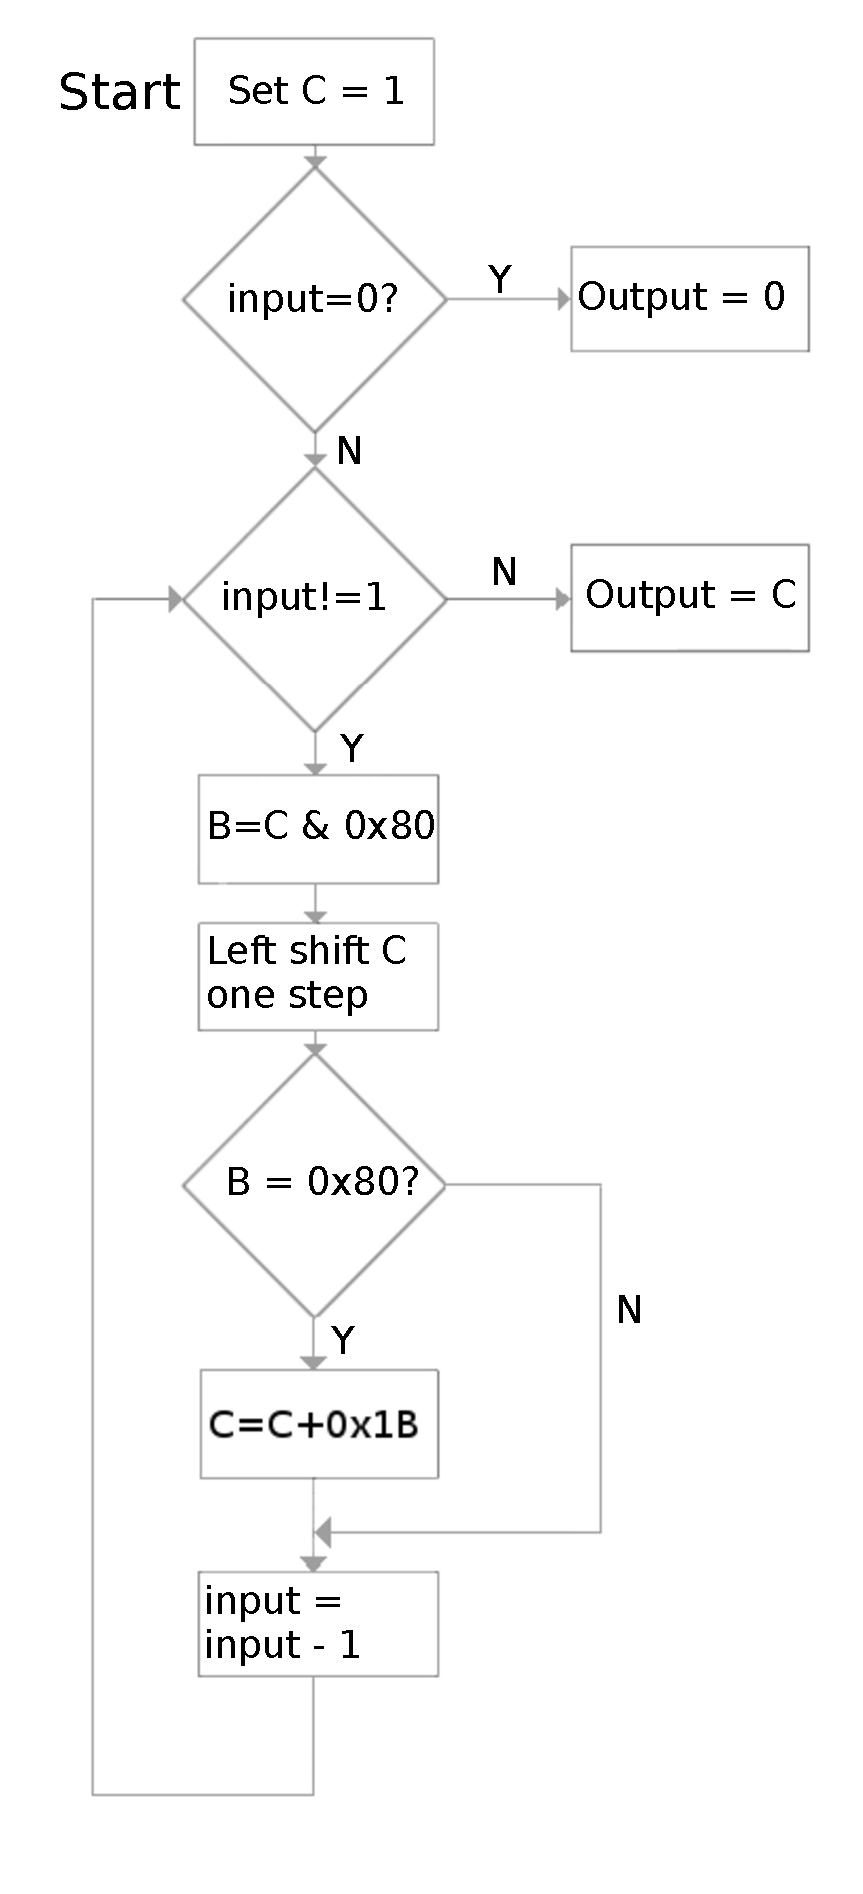
\includegraphics[height=0.6\textheight]{flowchart}
  \end{center}
  \caption{Flowchart of the Rcon function}
  \label{img:rcon}
\end{figure}

\begin{figure}
  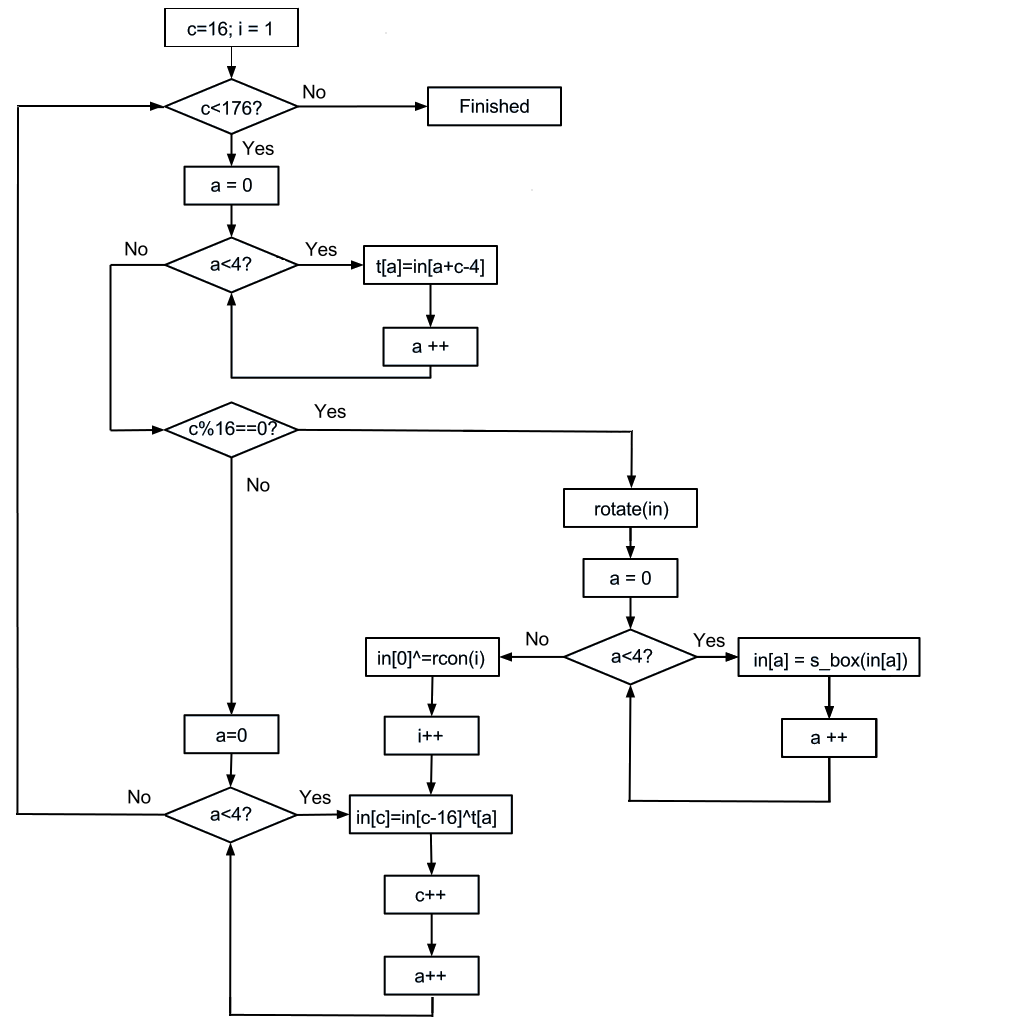
\includegraphics[width=\textwidth]{keyschedule}
  \caption{Flowchart of the key schedule}
  \label{img:keysch}
\end{figure}


